\documentclass[a4paper, 12pt]{article}

% packages
\usepackage{amssymb}
\usepackage[fleqn]{mathtools}
\usepackage{tikz}
\usepackage{enumerate}
\usepackage{bussproofs}
\usepackage{xcolor}
\usepackage[margin=1.3cm]{geometry}
\usepackage{logicproof}
\usepackage{diagbox}
\usepackage{listings}
\usepackage{graphicx}
\usepackage{lstautogobble}
\usepackage{hyperref}
\usepackage{multirow}
\usepackage{tipa}
\usepackage{pgfplots}
\usepackage{adjustbox}

% tikz libraries
\usetikzlibrary{
    decorations.pathreplacing,
    arrows,
    shapes,
    shapes.gates.logic.US,
    circuits.logic.US,
    calc,
    automata,
    positioning,
    intersections
}

\pgfplotsset{compat=1.16}

\pgfmathdeclarefunction{gauss}{2}{%
  \pgfmathparse{1/(#2*sqrt(2*pi))*exp(-((x-#1)^2)/(2*#2^2))}%
}

\allowdisplaybreaks % allow environments to break
\setlength\parindent{0pt} % no indent

% shorthand for verbatim
% this clashes with logicproof, so maybe fix this at some point?
\catcode`~=\active
\def~#1~{\texttt{#1}}

% code listing
\lstdefinestyle{main}{
    numberstyle=\tiny,
    breaklines=true,
    showspaces=false,
    showstringspaces=false,
    tabsize=2,
    numbers=left,
    basicstyle=\ttfamily,
    columns=fixed,
    fontadjust=true,
    basewidth=0.5em,
    autogobble,
    xleftmargin=3.0ex,
    mathescape=true
}
\newcommand{\dollar}{\mbox{\textdollar}} %
\lstset{style=main}

% augmented matrix
\makeatletter
\renewcommand*\env@matrix[1][*\c@MaxMatrixCols c]{%
\hskip -\arraycolsep
\let\@ifnextchar\new@ifnextchar
\array{#1}}
\makeatother

% ceiling / floor
\DeclarePairedDelimiter{\ceil}{\lceil}{\rceil}
\DeclarePairedDelimiter{\floor}{\lfloor}{\rfloor}

% custom commands
\newcommand{\indefint}[2]{\int #1 \, \mathrm{d}#2}
\newcommand{\defint}[4]{\int_{#1}^{#2} #3 \, \mathrm{d}#4}
\newcommand{\pdif}[2]{\frac{\partial #1}{\partial #2}}
\newcommand{\dif}[2]{\frac{\mathrm{d}#1}{\mathrm{d}#2}}
\newcommand{\limit}[2]{\raisebox{0.5ex}{\scalebox{0.8}{$\displaystyle{\lim_{#1 \to #2}}$}}}
\newcommand{\limitsup}[2]{\raisebox{0.5ex}{\scalebox{0.8}{$\displaystyle{\limsup_{#1 \to #2}}$}}}
\newcommand{\summation}[2]{\sum\limits_{#1}^{#2}}
\newcommand{\product}[2]{\prod\limits_{#1}^{#2}}
\newcommand{\intbracket}[3]{\left[#3\right]_{#1}^{#2}}
\newcommand{\laplace}{\mathcal{L}}
\newcommand{\fourier}{\mathcal{F}}
\newcommand{\mat}[1]{\boldsymbol{#1}}
\renewcommand{\vec}[1]{\boldsymbol{#1}}
\newcommand{\rowt}[1]{\begin{bmatrix}
    #1
\end{bmatrix}^\top}
\DeclareMathOperator*{\argmax}{argmax}
\DeclareMathOperator*{\argmin}{argmin}

\newcommand{\lto}[0]{\leadsto\ }

\newcommand{\ulsmash}[1]{\underline{\smash{#1}}}

\newcommand{\powerset}[0]{\wp}
\renewcommand{\emptyset}[0]{\varnothing}

\makeatletter
\newsavebox{\@brx}
\newcommand{\llangle}[1][]{\savebox{\@brx}{\(\m@th{#1\langle}\)}%
  \mathopen{\copy\@brx\kern-0.5\wd\@brx\usebox{\@brx}}}
\newcommand{\rrangle}[1][]{\savebox{\@brx}{\(\m@th{#1\rangle}\)}%
  \mathclose{\copy\@brx\kern-0.5\wd\@brx\usebox{\@brx}}}
\makeatother
\newcommand{\lla}{\llangle}
\newcommand{\rra}{\rrangle}
\newcommand{\la}{\langle}
\newcommand{\ra}{\rangle}
\newcommand{\crnr}[1]{\text{\textopencorner} #1 \text{\textcorner}}
\newcommand{\bnfsep}[0]{\ |\ }
\newcommand{\concsep}[0]{\ ||\ }

\newcommand{\axiom}[1]{\AxiomC{#1}}
\newcommand{\unary}[1]{\UnaryInfC{#1}}
\newcommand{\binary}[1]{\BinaryInfC{#1}}
\newcommand{\trinary}[1]{\TrinaryInfC{#1}}
\newcommand{\quaternary}[1]{\QuaternaryInfC{#1}}
\newcommand{\quinary}[1]{\QuinaryInfC{#1}}
\newcommand{\dproof}[0]{\DisplayProof}
\newcommand{\llabel}[1]{\LeftLabel{\scriptsize #1}}
\newcommand{\rlabel}[1]{\RightLabel{\scriptsize #1}}

\newcommand{\ttbs}{\char`\\}
\newcommand{\lrbt}[0]{\ \bullet\ }

% colours
\newcommand{\violet}[1]{\textcolor{violet}{#1}}
\newcommand{\blue}[1]{\textcolor{blue}{#1}}
\newcommand{\red}[1]{\textcolor{red}{#1}}
\newcommand{\teal}[1]{\textcolor{teal}{#1}}

% reasoning proofs
\usepackage{ltablex}
\usepackage{environ}
\keepXColumns
\NewEnviron{reasoning}{
    \begin{tabularx}{\textwidth}{rlX}
        \BODY
    \end{tabularx}
}
\newcommand{\proofline}[3]{$(#1)$ & $#2$ & \hfill #3 \smallskip \\}
\newcommand{\proofarbitrary}[1]{& take arbitrary $#1$ \smallskip \\}
\newcommand{\prooftext}[1]{\multicolumn{3}{l}{#1} \smallskip \\}
\newcommand{\proofmath}[3]{$#1$ & = $#2$ & \hfill #3 \smallskip \\}
\newcommand{\prooftherefore}[1]{& $\therefore #1$ \smallskip \\}
\newcommand{\proofbc}[0]{\prooftext{\textbf{Base Case}}}
\newcommand{\proofis}[0]{\prooftext{\textbf{Inductive Step}}}

% ER diagrams
\newcommand{\nattribute}[4]{
    \node[draw, state, inner sep=0cm, minimum size=0.2cm, label=#3:{#4}] (#1) at (#2) {};
}
\newcommand{\mattribute}[4]{
    \node[draw, state, accepting, inner sep=0cm, minimum size=0.2cm, label=#3:{#4}] (#1) at (#2) {};
}
\newcommand{\dattribute}[4]{
    \node[draw, state, dashed, inner sep=0cm, minimum size=0.2cm, label=#3:{#4}] (#1) at (#2) {};
}
\newcommand{\entity}[3]{
    \node[] (#1-c) at (#2) {#3};
    \node[inner sep=0cm] (#1-l) at ($(#1-c) + (-1, 0)$) {};
    \node[inner sep=0cm] (#1-r) at ($(#1-c) + (1, 0)$) {};
    \node[inner sep=0cm] (#1-u) at ($(#1-c) + (0, 0.5)$) {};
    \node[inner sep=0cm] (#1-d) at ($(#1-c) + (0, -0.5)$) {};
    \draw
    ($(#1-c) + (-1, 0.5)$) -- ($(#1-c) + (1, 0.5)$) -- ($(#1-c) + (1, -0.5)$) -- ($(#1-c) + (-1, -0.5)$) -- cycle;
}
\newcommand{\relationship}[3]{
    \node[] (#1-c) at (#2) {#3};
    \node[inner sep=0cm] (#1-l) at ($(#1-c) + (-1, 0)$) {};
    \node[inner sep=0cm] (#1-r) at ($(#1-c) + (1, 0)$) {};
    \node[inner sep=0cm] (#1-u) at ($(#1-c) + (0, 1)$) {};
    \node[inner sep=0cm] (#1-d) at ($(#1-c) + (0, -1)$) {};
    \draw
    ($(#1-c) + (-1, 0)$) -- ($(#1-c) + (0, 1)$) -- ($(#1-c) + (1, 0)$) -- ($(#1-c) + (0, -1)$) -- cycle;
}

% AVL Trees
\newcommand{\avltri}[4]{
    \draw ($(#1)$) -- ($(#1) + #4*(0.5, -1)$) -- ($(#1) + #4*(-0.5, -1)$) -- cycle;
    \node at ($(#1) + #4*(0, -1) + (0, 0.5)$) {#3};
    \node at ($(#1) + #4*(0, -1) + (0, -0.5)$) {#2};
}

% RB Trees
\tikzset{rbtr/.style={inner sep=2pt, circle, draw=black, fill=red}}
\tikzset{rbtb/.style={inner sep=2pt, circle, draw=black, fill=black}}

% Samples
\tikzset{spos/.style={inner sep=2pt, circle, draw=black, fill=blue!20}}
\tikzset{sneg/.style={inner sep=2pt, circle, draw=black, fill=red!20}}

% Joins
\newcommand\ljoin{\stackrel{\mathclap{\normalfont\mbox{\tiny L}}}{\bowtie}}
\newcommand\rjoin{\stackrel{\mathclap{\normalfont\mbox{\tiny R}}}{\bowtie}}
\newcommand\ojoin{\stackrel{\mathclap{\normalfont\mbox{\tiny O}}}{\bowtie}}

\setcounter{MaxMatrixCols}{100}

% actual document
\begin{document}
    {\sc Computing $3^\text{rd}$ Year Notes} \hfill ~https://github.com/lin-e/imperial-revision~
    \rule{\textwidth}{0.1pt}
    \section*{CO317 - Graphics \hfill (60005)}
        \subsection*{Lecture 1 - Projections and Transformations}
            \subsubsection*{Two Dimensional Graphics}
                At the lowest level, in every operating system, graphics processing operates on the pixels in a window with primitives, such as;
                \begin{itemize}
                    \itemsep0em
                    \item ~SetPixel(int x, int y, int colour);~
                    \item ~DrawLine(int xs, int ys, int xf, int yf);~
                \end{itemize}
                However, we'd like to be able to draw scenes from a three-dimensional world and have it appear in two-dimensional graphics primitives.
            \subsubsection*{World Coordinate System}
                In order to achieve independence when drawing objects, we define a world coordinate system.
                For example, let our world be defined in meters, we can then allow a pixel to represent a millimetre.
                A viewing area is a window, and is defined as part of our 3D world.
                \textbf{Clipping} occurs when we attempt to draw outside (dashed) of the \violet{window};
                \begin{lstlisting}
                    SetWindow(30, 10, 70, 50)
                    DrawLine(40, 3, 90, 30)
                    DrawLine(50, 60, 60, 40)
                \end{lstlisting}
                \begin{center}
                    \begin{tikzpicture}[x=0.075cm, y=0.075cm]
                        \draw (0, 0) edge[->] (0, 55);
                        \draw (0, 0) edge[->] (75, 0);

                        \draw[violet] (30, 10) -- (30, 50) -- (70, 50) -- (70, 10) -- cycle;
                        \draw[dashed]
                        (0, 10) -- (30, 10)
                        (0, 50) -- (30, 50)
                        (30, 0) -- (30, 10)
                        (70, 0) -- (70, 10);

                        \draw[dashed]
                        (40, 3) -- (52.963, 10)
                        (70, 19.2) -- (90, 30);
                        \draw (52.963, 10) -- (70, 19.2);

                        \draw[dashed] (50, 60) -- (55, 50);
                        \draw (55, 50) -- (60, 40);

                        \node at (-10, 10) {10};
                        \node at (-10, 50) {50};
                        \node at (30, -10) {30};
                        \node at (70, -10) {70};
                    \end{tikzpicture}
                \end{center}
                However, this isn't as trivial to do in 3D, as it cannot simply be left to the operating system.
                While we can represent 3D objects as a series of 2D commands, it's inefficient and expensive for the OS to perform the clipping (therefore we should do this manually).
            \subsubsection*{Normalisation}
                A normalisation process is required to convert from device independent commands (where screen resolution isn't taken into account) to drawing commands using pixels.
                Consider a point in the world coordinate window $(X_w, Y_w)$, and its corresponding result on the viewport (pixel coordinates; $(X_v, Y_v)$);
                \begin{center}
                    \begin{tikzpicture}[x=0.66cm, y=0.66cm]
                        \draw[rounded corners] (0, 0) -- (16, 0) -- (16, 9) -- (0, 9) -- cycle;

                        \draw (2, 2) -- (6, 2) -- (6, 6) -- (2, 6) -- cycle;
                        \node[rbtb] at (3, 3.5) {};
                        \node at (4, 4) {$(X_v, Y_v)$};

                        \begin{scope}[shift={(-9, 3)}]
                            \draw (0, 0) -- (6, 0) -- (6, 6) -- (0, 6) -- cycle;
                            \node[rbtb] at (1.5, 2.25) {};
                            \node at (2.5, 2.75) {$(X_w, Y_w)$};
                        \end{scope}

                        \draw[dashed]
                        (-9, 3) -- (2, 2)
                        (-3, 3) -- (6, 2)
                        (-3, 9) -- (6, 6)
                        (-9, 9) -- (2, 6)
                        (-9, 3) -- (-9, 0)
                        (-3, 3) -- (-3, 0)
                        (2, 2) -- (2, 0)
                        (6, 2) -- (6, 0);

                        \node at (-9, -1) {$W_{xmin}$};
                        \node at (-3, -1) {$W_{xmax}$};
                        \node at (2, -1) {$V_{xmin}$};
                        \node at (6, -1) {$V_{xmax}$};
                    \end{tikzpicture}
                \end{center}
                The expressions are similar for $Y$;
                $$\frac{(X_w - W_{xmin})}{(W_{xmax} - W_{xmin})} = \frac{(X_v - V_{xmin})}{(V_{xmax} - V_{xmin})} \Rightarrow X_v = \frac{(X_w - W_{xmin})(V_{xmax} - V_{xmin})}{(W_{xmax} - W_{xmin})} + V_{xmin}$$
                This gives us the resulting pair of linear equations (intuitively), where the constants found from the known values $W_{xmin}, V_{xmax}$, etc. are used to define the normalisation;
                \begin{align*}
                    X_v & = AX_w + B \\
                    Y_v & = CY_w + D
                \end{align*}
            \subsubsection*{Polygon Rendering}
                Most graphics applications deal with very simple objects - flat / planar polyhedra, referred to as \textbf{faces} or \textbf{facets}.
                These are graphic primitives, and can be used to approximate any shape.
                Consider the following tetrahedron, consisting of four vertices;
                \begin{center}
                    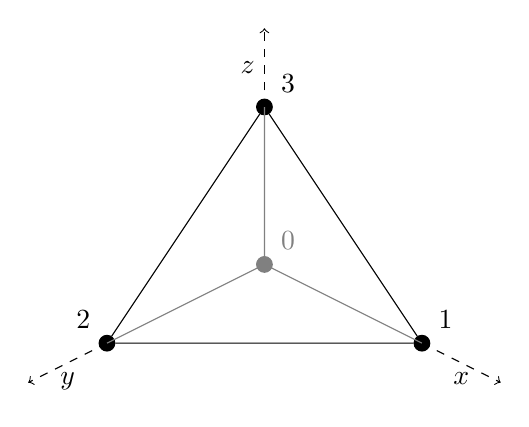
\begin{tikzpicture}
                        \node[inner sep=2pt, circle, draw=black!50, fill=black!50] at (0, 0) {};
                        \node[rbtb] (n3) at (0, 2) {};
                        \node[rbtb] (n1) at (2, -1) {};
                        \node[rbtb] (n2) at (-2, -1) {};

                        \node[black!50] at (0.3, 0.3) {0};
                        \node at (0.3, 2.3) {3};
                        \node at (2.3, -0.7) {1};
                        \node at (-2.3, -0.7) {2};

                        \draw[black!50]
                        (0, 0) -- (0, 2)
                        (0, 0) -- (2, -1)
                        (0, 0) -- (-2, -1);

                        \draw
                        (0, 2) edge[dashed, ->, left] node{$z$} (0, 3)
                        (2, -1) edge[dashed, ->, below] node{$x$} (3, -1.5)
                        (-2, -1) edge[dashed, ->, below] node{$y$} (-3, -1.5)
                        (n3) -- (n1) -- (n2) -- (n3);
                    \end{tikzpicture}
                \end{center}
                For this, we need a mixture of different data, including numerical data about the actual 3D coordinates of the vertices, as well as topological data regarding what vertices are connected to what.
                This can be represented in the following tables;
                \begin{center}
                    \hfill
                    \begin{tabular}{c|c}
                        \multicolumn{2}{c}{vertex data} \\
                        \hline
                        index & location \\
                        \hline
                        $0$ & $(0, 0, 0)$ \\
                        $1$ & $(1, 0, 0)$ \\
                        $2$ & $(0, 1, 0)$ \\
                        $3$ & $(0, 0, 1)$
                    \end{tabular}
                    \hfill
                    \begin{tabular}{c|c}
                        \multicolumn{2}{c}{face data} \\
                        \hline
                        index & vertices \\
                        \hline
                        $0$ & 0 1 3 \\
                        $1$ & 0 2 1 \\
                        $2$ & 0 3 2 \\
                        $3$ & 1 2 3
                    \end{tabular}
                    \hfill \phantom{}
                \end{center}
                This separation allows for the vertices to move without affecting the faces.
            \subsubsection*{Projections}
                In order to draw a 3D wire frame, the points must first be converted into a 2D representation, via a \textbf{projection}, which can then be drawn with simple drawing primitives.
                Intuitively, we have an observer (a focal point) where all viewing rays converge.
                The observer is located between a projection surface $P$ and an object $V$.
                While it's possible to project onto any surface, we only consider linear projections onto a flat surface.
            \subsubsection*{Orthographic Projections}
                The simplest form of a projection is an \textbf{orthographic projection}.
                The assumptions made are that the viewpoint is located at $z = -\infty$, and the plane of projection is $z = 0$.
                With the viewing point being infinitely far away, the rays become parallel.
                This gives all projectors the same direction;
                $$\vec{d} = \begin{bmatrix}
                    0 \\ 0 \\ -1
                \end{bmatrix}$$
                This gives the following, with each projection line having the equation $\vec{P} = \vec{V} + \mu \vec{d}$;
                \begin{center}
                    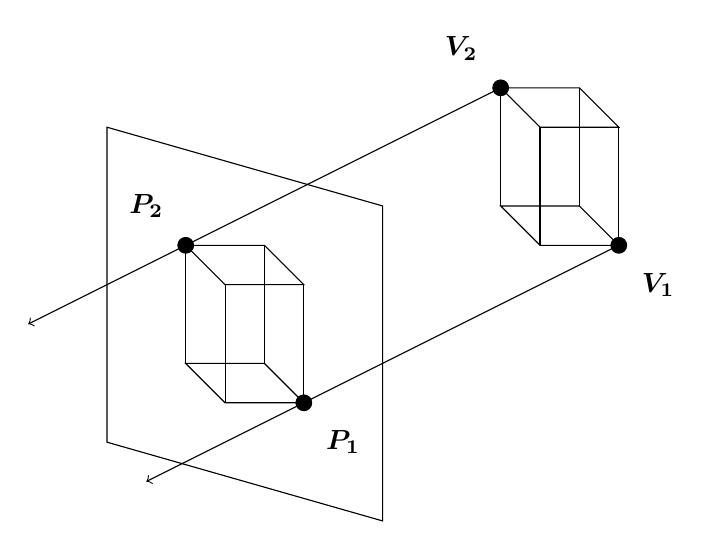
\begin{tikzpicture}
                        \draw (-1, 1.5) -- (2.5, 0.5) -- (2.5, -3.5) -- (-1, -2.5) -- cycle;
                        \begin{scope}[shift={(0, 0)}]
                            \draw (0, 0) -- (1, 0) -- (1.5, -0.5) -- (0.5, -0.5) -- cycle;
                            \draw (0, -1.5) -- (1, -1.5) -- (1.5, -2) -- (0.5, -2) -- cycle;
                            \draw
                            (0, 0) -- (0, -1.5)
                            (1, 0) -- (1, -1.5)
                            (1.5, -0.5) -- (1.5, -2)
                            (0.5, -0.5) -- (0.5, -2);
                        \end{scope}
                        \begin{scope}[shift={(4, 2)}]
                            \draw (0, 0) -- (1, 0) -- (1.5, -0.5) -- (0.5, -0.5) -- cycle;
                            \draw (0, -1.5) -- (1, -1.5) -- (1.5, -2) -- (0.5, -2) -- cycle;
                            \draw
                            (0, 0) -- (0, -1.5)
                            (1, 0) -- (1, -1.5)
                            (1.5, -0.5) -- (1.5, -2)
                            (0.5, -0.5) -- (0.5, -2);
                        \end{scope}

                        \draw
                        (4, 2) edge[->] (-2, -1)
                        (5.5, 0) edge[->] (-0.5, -3);

                        \node[rbtb] at (4, 2) {};
                        \node[rbtb] at (5.5, 0) {};
                        \node[rbtb] at (0, 0) {};
                        \node[rbtb] at (1.5, -2) {};

                        \node at (3.5, 2.5) {$\vec{V_2}$};
                        \node at (6, -0.5) {$\vec{V_1}$};
                        \node at (-0.5, 0.5) {$\vec{P_2}$};
                        \node at (2, -2.5) {$\vec{P_1}$};
                    \end{tikzpicture}
                \end{center}
                By substituting in the direction $\vec{d}$ we have determined, it gives the following Cartesian equations for each component;
                \begin{align*}
                    P_x & = V_x + 0 \\
                    P_y & = V_y + 0 \\
                    P_z & = V_z - \mu \\
                \end{align*}
                However, since we have the projection plane $z = 0$, we also know that $P_z = 0$, therefore we don't need to solve for $\mu$.
                From this, we can determine the projected location is the 3D $x$ and $y$ components of the vertex;
                $$\vec{P} = \begin{bmatrix}
                    V_x \\ V_y \\ 0
                \end{bmatrix}$$
                Viewing the wireframe for a cube directly from a face would look like the following;
                \begin{center}
                    \begin{tikzpicture}[x=1.5cm, y=1.5cm]
                        \draw (0, 0) -- (1, 0) -- (1, 1) -- (0, 1) -- cycle;
                    \end{tikzpicture}
                \end{center}
            \subsubsection*{Perspective Projection}
                While orthographic projections are fine when depth isn't a consideration (such as objects mostly being at the same distance from the viewer), it's insufficient for close work, where we want details to be realistic.
                The difference here is that we are no longer at an infinite distance (instead being at the origin), and the projection plane is $z = f$ (where $f$ stands for focal length);
                \begin{center}
                    \begin{tikzpicture}
                        \draw
                        (0, 0) edge[->] (10, 0)
                        (0, 0) edge[->] (0, 7);
                        \node at (-0.5, 7) {$y$};
                        \node at (10, -0.5) {$x$};
                        \node at (9, 4) {$z$};

                        \draw (2, 1) -- (2, 4) -- (6, 4) -- (6, 1) -- cycle;
                        \draw
                        (0, 0) -- (2, 1)
                        (2, 1) edge[dashed] (6, 3)
                        (6, 3) edge[->] (9, 4.5);

                        \draw (5, 7) -- (7, 6) -- (5.5, 5) -- cycle;
                        \node[rbtb] at (5, 7) {};
                        \node[rbtb] at (7, 6) {};
                        \node at (4.5, 7) {$\vec{V_1}$};
                        \node at (7.5, 6) {$\vec{V_2}$};

                        \draw (2.5, 3.5) -- (3.5, 3) -- (2.75, 2.5) -- cycle;
                        \node[rbtb] at (2.5, 3.5) {};
                        \node[rbtb] at (3.5, 3) {};
                        \node at (2, 3.5) {$\vec{P_1}$};
                        \node at (4, 3) {$\vec{P_2}$};

                        \draw[black!50]
                        (5, 7) -- (0, 0)
                        (7, 6) -- (0, 0);

                        \draw
                        (0, 0) edge[dashed] (0, -2)
                        (2, 1) edge[dashed] (2, -1)
                        (0, -1.5) edge[<->, below] node{$f$} (2, -0.5);
                    \end{tikzpicture}
                \end{center}
                This gives us the following equation (since all projectors must go through the origin);
                $$\vec{P} = \mu \vec{V}$$
                We can work out the value of $\mu$, let it be $\mu_p$ as follows;
                \begin{align*}
                    P_z & = f & \text{by projection plane} \\
                    \mu_p & = \frac{P_z}{V_z} \\
                    & = \frac{f}{V_z} \\
                    P_x & = \mu_p V_x \\
                    & = \frac{f V_x}{V_z} \\
                    P_y & = \mu_p V_y \\
                    & = \frac{f V_y}{V_z}
                \end{align*}
                Viewing the wireframe for a cube directly from a face would look like the following (note the difference to the orthographic projection);
                \begin{center}
                    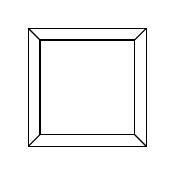
\begin{tikzpicture}[x=1.5cm, y=1.5cm]
                        \draw (0, 0) -- (1, 0) -- (1, 1) -- (0, 1) -- cycle;
                        \draw (0.1, 0.1) -- (0.9, 0.1) -- (0.9, 0.9) -- (0.1, 0.9) -- cycle;
                        \draw
                        (0, 0) -- (0.1, 0.1)
                        (1, 0) -- (0.9, 0.1)
                        (1, 1) -- (0.9, 0.9)
                        (0, 1) -- (0.1, 0.9);
                    \end{tikzpicture}
                \end{center}
            \subsubsection*{Transformations}
                Scenes are defined in a particular coordinate system, but we want to be able to draw a scene from any angle.
                To do so, it's easier to have the viewpoint at the origin, and the $z$-axis as the direction of view.
                As such, we need to be able to \textbf{transform} the coordinates of a scene.
                \begin{center}
                    \begin{tikzpicture}
                        \begin{scope}[shift={(0, 0)}]
                            \draw
                            (0, 0) edge[->, below] node{$x$} (5, 0)
                            (0, 0) edge[->, left] node{$y$} (0, 2)
                            (0, 0) edge[->, above] node{$z$} (2, 1);

                            \begin{scope}[shift={(2.5, 0.75)}]
                                \draw (0, 0) -- (1, 0) -- (1, 1) -- (0, 1) -- cycle;
                                \draw
                                (0, 0) -- (0.5, 0.5)
                                (1, 0) -- (1.5, 0.5)
                                (1, 1) -- (1.5, 1.5)
                                (0, 1) -- (0.5, 1.5);
                                \draw (0.5, 0.5) -- (1.5, 0.5) -- (1.5, 1.5) -- (0.5, 1.5) -- cycle;
                            \end{scope}

                            \draw
                            (0, 0) edge[dashed, ->, below] node{$C_x$} (4, 0)
                            (4, 0) edge[dashed, ->, right] node{\ \ $C_z$} (6, 1)
                            (6, 1) edge[dashed, ->, right] node{$C_y$} (6, 3)
                            (6, 3) edge[->, above] node{$\vec{d}$} (5, 2.5);

                            \node at (6.5, 3) {$\vec{C}$};
                            \node at (-0.5, 0) {$\vec{O}$};
                        \end{scope}
                        \begin{scope}[shift={(8, 0)}]
                            \draw
                            (0, 0) edge[dashed] (5, 0)
                            (0, 0) edge[dashed] (0, 2)
                            (0, 0) edge[dashed] (2, 1);

                            \begin{scope}[shift={(2.5, 0.75)}]
                                \draw (0, 0) -- (1, 0) -- (1, 1) -- (0, 1) -- cycle;
                                \draw
                                (0, 0) -- (0.5, 0.5)
                                (1, 0) -- (1.5, 0.5)
                                (1, 1) -- (1.5, 1.5)
                                (0, 1) -- (0.5, 1.5);
                                \draw (0.5, 0.5) -- (1.5, 0.5) -- (1.5, 1.5) -- (0.5, 1.5) -- cycle;
                            \end{scope}

                            \draw
                            (6, 3) edge[->, below] node{$z$} (5, 2.5)
                            (6, 3) edge[->, right] node{$y$} (5.5, 4)
                            (6, 3) edge[->, below] node{$x$} (5.25, 3.5);

                            \node at (6.5, 3) {$\vec{O}$};
                        \end{scope}
                    \end{tikzpicture}
                \end{center}
                These are done by the application of transformation matrices.
                For example, a standard transformation to make an object twice as big from the origin;
                $$\begin{bmatrix}
                    x^\prime \\ y^\prime \\ z^\prime
                \end{bmatrix} = \begin{bmatrix}
                    2 & 0 & 0 \\
                    0 & 2 & 0 \\
                    0 & 0 & 2
                \end{bmatrix} \begin{bmatrix}
                    x \\ y \\ z
                \end{bmatrix}$$
            \subsubsection*{Translation}
                However, being restricted to matrix operations with $\mathbb{R}^{3 \times 3}$ means that we cannot represent translations (for example, a shift of two units on the $x$-axis, such that $x^\prime = x + 2$).
                The solution to this is to use 4D \textbf{homogenous coordinates}, where we assume the fourth dimension is fixed to 1.
                $$\begin{bmatrix}
                    x^\prime \\ y^\prime \\ z^\prime \\ 1
                \end{bmatrix} = \begin{bmatrix}
                    1 & 0 & 0 & 2 \\
                    0 & 1 & 0 & 0 \\
                    0 & 0 & 1 & 0 \\
                    0 & 0 & 0 & 1
                \end{bmatrix} \begin{bmatrix}
                    x \\ y \\ z \\ 1
                \end{bmatrix}$$
                Frequently the last ordinate is 1, however in general it is a scale factor;
                $$\underbrace{(p_x, p_y, p_z, s)}_\text{homogenous} \Leftrightarrow \underbrace{\left(\frac{p_x}{s}, \frac{p_y}{s}, \frac{p_z}{s}\right)}_\text{Cartesian}$$
            \subsubsection*{Affine Transformations}
                Affine transformations preserve parallel lines.
                Most of the transformations we require are affine, with the most important being scaling, rotation, and translation;
                \begin{itemize}
                    \itemsep0em
                    \item \textbf{scaling} \hfill by $(s_x, s_y, s_z)$
                        $$\begin{bmatrix}
                            s_x & 0 & 0 & 1 \\
                            0 & s_y & 0 & 1 \\
                            0 & 0 & s_z & 1 \\
                            0 & 0 & 0 & 1
                        \end{bmatrix} \begin{bmatrix}
                            p_x \\ p_y \\ p_z \\ 1
                        \end{bmatrix} = \begin{bmatrix}
                            s_x p_x \\
                            s_y p_y \\
                            s_z p_z \\
                            1
                        \end{bmatrix}$$
                    \item \textbf{rotation}
                        \smallskip

                        In order to define a rotation, we need both an axis and an angle, with the simplest rotations being about the Cartesian axes.
                        The following matrices are used for rotations of $\theta$ about each of the axes;
                        \begin{align*}
                            \mat{\mathcal{R}_x} & = \begin{bmatrix}
                                1 & 0 & 0 & 0 \\
                                0 & \cos \theta & -\sin \theta & 0 \\
                                0 & \sin \theta & \cos \theta & 0 \\
                                0 & 0 & 0 & 1
                            \end{bmatrix} \\
                            \mat{\mathcal{R}_y} & = \begin{bmatrix}
                                \cos \theta & 0 & \sin \theta & 0 \\
                                0 & 1 & 0 & 0 \\
                                -\sin \theta & 0 & \cos \theta & 0 \\
                                0 & 0 & 0 & 1
                            \end{bmatrix} \\
                            \mat{\mathcal{R}_z} & = \begin{bmatrix}
                                \cos \theta & -\sin \theta & 0 & 0 \\
                                \sin \theta & \cos \theta & 0 & 0 \\
                                0 & 0 & 1 & 0 \\
                                0 & 0 & 0 & 1
                            \end{bmatrix}
                        \end{align*}
                        It's important to note that \textbf{rotations have a direction}.
                        In this course, we use a left-handed coordinate system, where the rotation is anti-clockwise when looking along the axis of rotation (think about the origin being closer to you, and the axis going off to $\infty$ away from you).
                    \item \textbf{translation} \hfill by $(t_x, t_y, t_z)$
                        $$\begin{bmatrix}
                            1 & 0 & 0 & t_x \\
                            0 & 1 & 0 & t_y \\
                            0 & 0 & 1 & t_z \\
                            0 & 0 & 0 & 1
                        \end{bmatrix} \begin{bmatrix}
                            p_x \\ p_y \\ p_z \\ 1
                        \end{bmatrix} = \begin{bmatrix}
                            p_x + t_x \\
                            p_y + t_y \\
                            p_z + t_z \\
                            1
                        \end{bmatrix}$$
                \end{itemize}
                However, perspective projections are an example of a non-affine transformation, as it doesn't preserve parallels.
                Intuitively, it's not invertible (singular), as we cannot convert from a photograph to a 3D model.
                \medskip

                Note that we should be careful when we combine transformation.
                As matrix multiplication isn't commutative, we should read a sequence of matrices multiplied together from right to left, with the right-most matrix, before the vector, being the \textbf{first} transformation to be applied.
        \subsection*{Lecture 2 - Transformations for Animation}
            Recall the transformation in the previous lecture, which took way too long to draw, moving the origin to the view point.
            It consists of three steps, with the latter two being used to align the $z$-axis with the view direction;
            \begin{enumerate}[1.]
                \itemsep0em
                \item translation of the origin \hfill fairly trivial to do
                    $$\mat{\mathcal{A}} = \begin{bmatrix}
                        1 & 0 & 0 & -C_x \\
                        0 & 1 & 0 & -C_y \\
                        0 & 0 & 1 & -C_z \\
                        0 & 0 & 0 & 1
                    \end{bmatrix}$$
                \item rotation about $y$-axis
                    \smallskip

                    Consider the following, looking at the $x-z$ plane;
                    \begin{center}
                        \begin{tikzpicture}[x=0.75cm, y=0.75cm]
                            \draw
                            (0, 0) edge[->] (0, 6)
                            (0, 0) edge[->] (6, 0)
                            (0, 0) edge[very thick, ->] (3, 4)
                            (0, 0) edge[very thick, ->] (0, 5)
                            (0, 0) edge[dashed, <->, below] node{$d_x$} (3, 0)
                            (3, 0) edge[dashed, <->, right] node{$d_z$} (3, 4);

                            \draw (0, 0) ++(53:1) arc (53:90:1);
                            \node at (0.4, 1.25) {$\theta$};

                            \node at (2.5, 4) {$\vec{v}$};
                            \node at (6, -0.5) {$x$};
                            \node at (-0.5, 6) {$z$};
                        \end{tikzpicture}
                    \end{center}
                    This can be used to calculate the following (note that here we are using a right-handed system);
                    \begin{align*}
                        || \vec{v} || & = v \\
                        & = \sqrt{d_x^2 + d_z^2} \\
                        \cos \theta & = \frac{d_z}{v} \\
                        \sin \theta & = \frac{d_x}{v} \\
                        \mat{\mathcal{B}} & = \begin{bmatrix}
                            \cos \theta & 0 & -\sin \theta & 0 \\
                            0 & 1 & 0 & 0 \\
                            -\sin \theta & 0 & \cos \theta & 0 \\
                            0 & 0 & 0 & 1
                        \end{bmatrix} \\
                        & = \begin{bmatrix}
                            \frac{d_z}{v} & 0 & -\frac{d_x}{v} & 0 \\
                            0 & 1 & 0 & 0 \\
                            \frac{d_x}{v} & 0 & \frac{d_z}{v} & 0 \\
                            0 & 0 & 0 & 1
                        \end{bmatrix}
                    \end{align*}
                \item rotation about $x$-axis
                    \smallskip

                    This follows a similar process, note that we are now aligned along the $y-z$ plane (for clarity, the horizontal distance is $v$);
                    \begin{center}
                        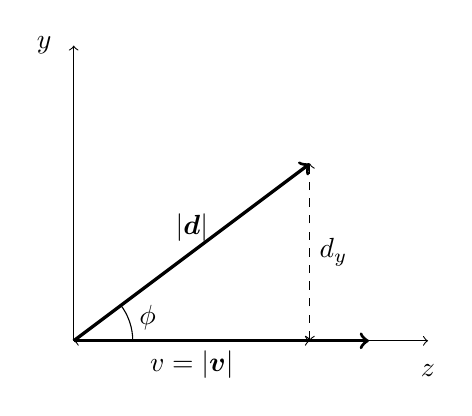
\begin{tikzpicture}[x=0.75cm, y=0.75cm]
                            \draw
                            (0, 0) edge[->] (6, 0)
                            (0, 0) edge[->] (0, 5)
                            (0, 0) edge[very thick, ->, above] node{$| \vec{d} |$} (4, 3)
                            (0, 0) edge[very thick, ->] (5, 0)
                            (0, 0) edge[dashed, <->, below] node{$v = | \vec{v} |$} (4, 0)
                            (4, 0) edge[dashed, <->, right] node{$d_y$} (4, 3);

                            \draw (0, 0) ++(38:1) arc (38:0:1);
                            \node at (1.25, 0.4) {$\phi$};
                            \node at (6, -0.5) {$z$};
                            \node at (-0.5, 5) {$y$};
                        \end{tikzpicture}
                    \end{center}
                    Similarly, the matrix can be obtained as follows;
                    \begin{align*}
                        \cos \phi & = \frac{v}{| \vec{d} |} \\
                        \sin \phi & = \frac{d_y}{| \vec{d} |} \\
                        \mat{\mathcal{C}} & = \begin{bmatrix}
                            1 & 0 & 0 & 0 \\
                            0 & \cos \phi & -\sin \phi & 0 \\
                            0 & \sin \phi & \cos \phi & 0 \\
                            0 & 0 & 0 & 1
                        \end{bmatrix} \\
                        & = \begin{bmatrix}
                            1 & 0 & 0 & 0 \\
                            0 & \frac{v}{| \vec{d} |} & -\frac{d_y}{| \vec{d} |} & 0 \\
                            0 & \frac{d_y}{| \vec{d} |} & \frac{v}{| \vec{d} |} & 0 \\
                            0 & 0 & 0 & 1
                        \end{bmatrix}
                    \end{align*}
            \end{enumerate}
            From this, we are able to combine the matrices into the following;
            $$\mat{\mathcal{T}} = \mat{\mathcal{C}} \mat{\mathcal{B}} \mat{\mathcal{A}}$$
            For every point $\vec{P}$ in the scene, we can obtain $\vec{P_t} = \mat{\mathcal{T}}\vec{P}$, with the view in \textbf{canonical} form, allowing us to apply the standard perspective or orthographic projection.
            \subsubsection*{Rotation About a General Line}
                Rotation of a scene around a general line can be done as a combination of transformations.
                The idea is similar, with the following three steps;
                \begin{enumerate}[1.]
                    \itemsep0em
                    \item making the line of rotation one of the Cartesian axes
                        \smallskip

                        This uses the matrices derived before, rotating the general line to be aligned with the $z$-axis.
                    \item perform the rotation
                        \smallskip

                        Standard rotation around the $z$-axis defined previously.
                    \item restore line to original place
                        \smallskip

                        Inversion of the initial matrices to revert rotation.
                \end{enumerate}
                This gives us the following full matrix;
                $$\mat{\mathcal{T}} = \underbrace{\mat{\mathcal{A}^{-1}} \mat{\mathcal{B}^{-1}} \mat{\mathcal{C}^{-1}}}_3 \underbrace{\mat{\mathcal{R}_z}}_2 \underbrace{\mat{\mathcal{C}} \mat{\mathcal{B}} \mat{\mathcal{A}}}_1$$
            \subsubsection*{Projection Matrices}
                For the canonical / orthographic projection, the matrix simply drops the $z$ component;
                \begin{align*}
                    \mat{\mathcal{M}_O} & = \begin{bmatrix}
                        1 & 0 & 0 & 0 \\
                        0 & 1 & 0 & 0 \\
                        0 & 0 & 0 & 0 \\
                        0 & 0 & 0 & 1
                    \end{bmatrix} \\
                    \mat{\mathcal{M}_O} \begin{bmatrix}
                        x \\ y \\ z \\ 1
                    \end{bmatrix} & = \begin{bmatrix}
                        x \\ y \\ 0 \\ 1
                    \end{bmatrix}
                \end{align*}
                This is clearly non-invertible, as we are losing information about one of the axes.
                An effect of this is that we must do any effects in 3D \textbf{before} applying the projection matrix.
                \medskip

                The perspective projection matrix can also be done in a similar way;
                \begin{align*}
                    \mat{\mathcal{M}_p} & = \begin{bmatrix}
                        1 & 0 & 0 & 0 \\
                        0 & 1 & 0 & 0 \\
                        0 & 0 & 1 & 0 \\
                        0 & 0 & \frac{1}{f} & 0
                    \end{bmatrix} \\
                    \mat{\mathcal{M}_p} \begin{bmatrix}
                        x \\ y \\ z \\ 1
                    \end{bmatrix} & = \begin{bmatrix}
                        x \\ y \\ z \\ \frac{z}{f}
                    \end{bmatrix} \\
                    & \rightarrow \begin{bmatrix}
                        \frac{fx}{z} \\
                        \frac{fy}{z} \\
                        f \\
                        1
                    \end{bmatrix} & \text{using the fourth ordinate as a scale factor}
                \end{align*}
                Note that homogenous coordinates and vectors fall into one of two types;
                \begin{enumerate}[1.]
                    \itemsep0em
                    \item \textbf{position vectors}
                        \smallskip

                        These have a non-zero final ordinate ($s > 0$) and can be normalised to Cartesian form.
                        If two position vectors are added, we instead obtain the mid-point;
                        $$\begin{bmatrix}
                            X_a \\ Y_a \\ Z_a \\ 1
                        \end{bmatrix} + \begin{bmatrix}
                            X_b \\ Y_b \\ Z_b \\ 1
                        \end{bmatrix} = \begin{bmatrix}
                            X_a + X_b \\
                            Y_a + Y_b \\
                            Z_a + Z_b \\
                            2
                        \end{bmatrix} = \begin{bmatrix}
                            \frac{X_a + X_b}{2} \\
                            \frac{Y_a + Y_b}{2} \\
                            \frac{Z_a + Z_b}{2} \\
                            1
                        \end{bmatrix}$$
                        This has no real meaning in geometry, but is a useful observation.
                    \item \textbf{direction vectors}
                        \smallskip

                        These have a zero in the final ordinate, and have a direction and magnitude.
                        If two direction vectors are added, we obtain a direction vector (following the normal addition rule);
                        $$\begin{bmatrix}
                            x_i \\ y_i \\ z_i \\ 0
                        \end{bmatrix} + \begin{bmatrix}
                            x_j \\ y_j \\ z_j \\ 0
                        \end{bmatrix} = \begin{bmatrix}
                            x_i + x_j \\
                            y_i + y_j \\
                            z_i + z_j \\
                            0
                        \end{bmatrix}$$
                        However, if a direction vector is added to a position vector, we obtain another position vector;
                        $$\begin{bmatrix}
                            X \\ Y \\ Z \\ 1
                        \end{bmatrix} + \begin{bmatrix}
                            x \\ y \\ z \\ 0
                        \end{bmatrix} = \begin{bmatrix}
                            X + x \\
                            Y + y \\
                            Z + z \\
                            1
                        \end{bmatrix}$$
                \end{enumerate}
            \subsubsection*{Structure of a Transformation Matrix}
                Note that the bottom row of such a matrix is \textbf{always} 0 0 0 1.
                We can decompose the columns of a transformation matrix into three direction vectors and one position vector.
                The three direction vectors are the new axes and the position vector is the new origin.
                $$\underbrace{\begin{bmatrix}
                    q_x & r_x & s_x & C_x \\
                    q_y & r_y & s_y & C_y \\
                    q_z & r_z & s_z & C_z \\
                    0 & 0 & 0 & 1
                \end{bmatrix}}_\text{matrix} \rightarrow \underbrace{\begin{bmatrix}
                    q_x \\ q_y \\ q_z \\ 0
                \end{bmatrix} \begin{bmatrix}
                    r_x \\ r_y \\ r_z \\ 0
                \end{bmatrix} \begin{bmatrix}
                    s_x \\ s_y \\ s_z \\ 0
                \end{bmatrix}}_\text{direction vectors} \underbrace{\begin{bmatrix}
                    C_x \\ C_y \\ C_z \\ 1
                \end{bmatrix}}_\text{position vector}$$
                When applying this transformation to a direction vector, where the last ordinate is zero, no \textbf{translation} is applied.
                On the other hand, if it is a position vector, where the last ordinate is 1, all vectors will have the same displacement.
                \medskip

                The following results can be proved by observing changes to the standard basis vectors, and the origin after applying the matrix;
                \begin{itemize}
                    \itemsep0em
                    \item $\vec{q}$ \hfill transformed $x$-axis
                    \item $\vec{r}$ \hfill transformed $y$-axis
                    \item $\vec{s}$ \hfill transformed $z$-axis
                    \item $\vec{C}$ \hfill transformed origin
                \end{itemize}
            \subsubsection*{Dot Product}
                We can consider the dot product as a projection;
                $$\vec{P} \cdot \vec{u} = | \vec{P} | | \vec{u} | \cos \theta$$
                Visually, we can see the dot product as the following;
                \begin{center}
                    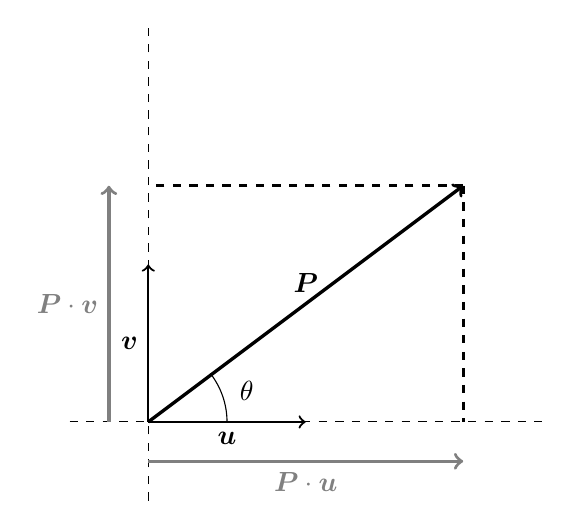
\begin{tikzpicture}
                        \draw
                        (-1, 0) edge[dashed] (5, 0)
                        (0, -1) edge[dashed] (0, 5)
                        (0, 0) edge[thick, ->, below] node{$\vec{u}$} (2, 0)
                        (0, 0) edge[thick, ->, left] node{$\vec{v}$} (0, 2)
                        (0, 0) edge[very thick, ->, above] node{$\vec{P}$} (4, 3)
                        (4, 3) edge[very thick, dashed] (0, 3)
                        (4, 3) edge[very thick, dashed] (4, 0);
                        \draw (0, 0) ++(38:1) arc (38:0:1);
                        \node at (1.25, 0.4) {$\theta$};
                        \draw[black!50]
                        (0, -0.5) edge[very thick, ->, below] node{$\vec{P} \cdot \vec{u}$} (4, -0.5)
                        (-0.5, 0) edge[very thick, ->, left] node{$\vec{P} \cdot \vec{v}$} (-0.5, 3);
                    \end{tikzpicture}
                \end{center}
                If $\vec{u}$ is along a co-ordinate axis, then $\vec{P} \cdot \vec{u}$ is the ordinate of $\vec{P}$ in the direction of $\vec{u}$.
                \medskip

                Consider changing to the new axes $\vec{u}, \vec{v}, \vec{w}$, and origin $\vec{C}$.
                We can call the first co-ordinate of $\vec{P}$ in the new system $\vec{P}_x^t$;
                \begin{align*}
                    \vec{P}_x^t & = (\vec{P} - \vec{C}) \cdot \vec{u} \\
                    & = \vec{P} \cdot \vec{u} - \vec{C} \cdot \vec{u}
                \end{align*}
                However, this can also be represented in matrix notation;
                $$\begin{bmatrix}
                    P_x^t \\
                    P_y^t \\
                    P_z^t \\
                    1
                \end{bmatrix} = \begin{bmatrix}
                    u_x & u_y & u_z & -\vec{C} \cdot \vec{u} \\
                    v_x & v_y & v_z & -\vec{C} \cdot \vec{v} \\
                    w_x & w_y & w_z & -\vec{C} \cdot \vec{w} \\
                    0 & 0 & 0 & 1
                \end{bmatrix} \begin{bmatrix}
                    P_x \\
                    P_y \\
                    P_z \\
                    1
                \end{bmatrix}$$
                Returning to the original problem, where we need to find a transformation matrix with a viewpoint $\vec{C}$ and direction $\vec{d}$.
                This can be done by first finding the vectors $\vec{u}, \vec{v}, \vec{w}$.
                Since $\vec{d}$ is the direction of the new axes, we can write (to get a unit vector);
                $$\vec{w} = \frac{\vec{d}}{| \vec{d} |}$$
                We also want to maintain an orthogonal basis, as well as all unit vectors.
                For the horizontal direction, we can write $\vec{u}$ in terms of some horizontal vector $\vec{p}$;
                \begin{align*}
                    \vec{u} & = \frac{\vec{p}}{| \vec{p} |} \\
                    p_y & = 0 & \text{ensure horizontal, no vertical component}
                \end{align*}
                Similarly, we want some vertical vector $\vec{q}$ to write $\vec{v}$;
                \begin{align*}
                    \vec{v} & = \frac{\vec{q}}{| \vec{q} |} \\
                    q_y & = 1 & \text{vertical, positive component}
                \end{align*}
                This gives us the following to solve;
                \begin{align*}
                    \vec{p} & = \begin{bmatrix}
                        p_x \\ 0 \\ p_z
                    \end{bmatrix} & \text{new horizontal} \\
                    \vec{q} & = \begin{bmatrix}
                        q_x \\ 1 \\ q_z
                    \end{bmatrix} & \text{new vertical}
                \end{align*}
                However, the view direction can also be written as the following (since we have the view direction, which happens to be the new $z$-axis as perpendicular to the remaining two vectors);
                $$\vec{d} = \vec{p} \times \vec{q}$$
                Using this, we can write $\vec{p}$ in terms of $\vec{q}$;
                \begin{align*}
                    \vec{d} & = \begin{bmatrix}
                        d_x \\ d_y \\ d_z
                    \end{bmatrix} \\
                    & = \vec{p} \times \vec{q} \\
                    & = \begin{vmatrix}
                        \vec{i} & \vec{j} & \vec{k} \\
                        p_x & 0 & p_z \\
                        q_x & 1 & q_z
                    \end{vmatrix} \\
                    & = -p_z \vec{i} + (p_z q_x - p_x q_z) \vec{j} + p_x \vec{k} \\
                    & = \begin{bmatrix}
                        -p_z \\
                        p_z q_x - p_x q_z \\
                        p_x
                    \end{bmatrix} & \Rightarrow \\
                    d_x & = -p_z \\
                    d_y & = p_z q_x - p_x q_z \\
                    d_z & = p_x & \Rightarrow \\
                    \vec{p} & = \begin{bmatrix}
                        d_z \\ 0 \\ -d_x
                    \end{bmatrix}
                \end{align*}
                However, since we know that the vectors $\vec{p}$ and $\vec{q}$ are orthogonal, we can say the following;
                \begin{align*}
                    \vec{p} \cdot \vec{q} & = 0 & \Rightarrow \\
                    p_x q_x + p_z q_z & = 0 \\
                    d_y & = p_z q_x - p_x q_z & \text{from above}
                \end{align*}
                Both of these equations can be fully written in terms of $\vec{d}$.
\end{document}